%%%%%%%%%%%%%%%%%%%%%%%%%%%%%%%%
% Compile with
% pdflatex --shell-escape -synctex=1 -interaction=nonstopmode partInCell.tex
% to convert it to png use:
% convert -density 300 -transparent white partInCell.pdf partInCell.png,
%%%%%%%%%%%%%%%%%%%%%%%%%%%%%%%%

\documentclass{standalone}

\usepackage[utf8]{inputenc}
\usepackage{tkz-fct}
\renewcommand{\familydefault}{\sfdefault}
\usepackage[scaled=1]{helvet}
\usepackage[helvet]{sfmath}
\everymath={\sf}
\usetikzlibrary{calc,arrows,intersections,angles,quotes,patterns}

\definecolor{AFLight}{HTML}{5CE0E6}
\definecolor{AFMiddle}{HTML}{51ADE5}
\definecolor{AFDark}{HTML}{0E4160}

\begin{document}

\tikzset{
   >=stealth
}
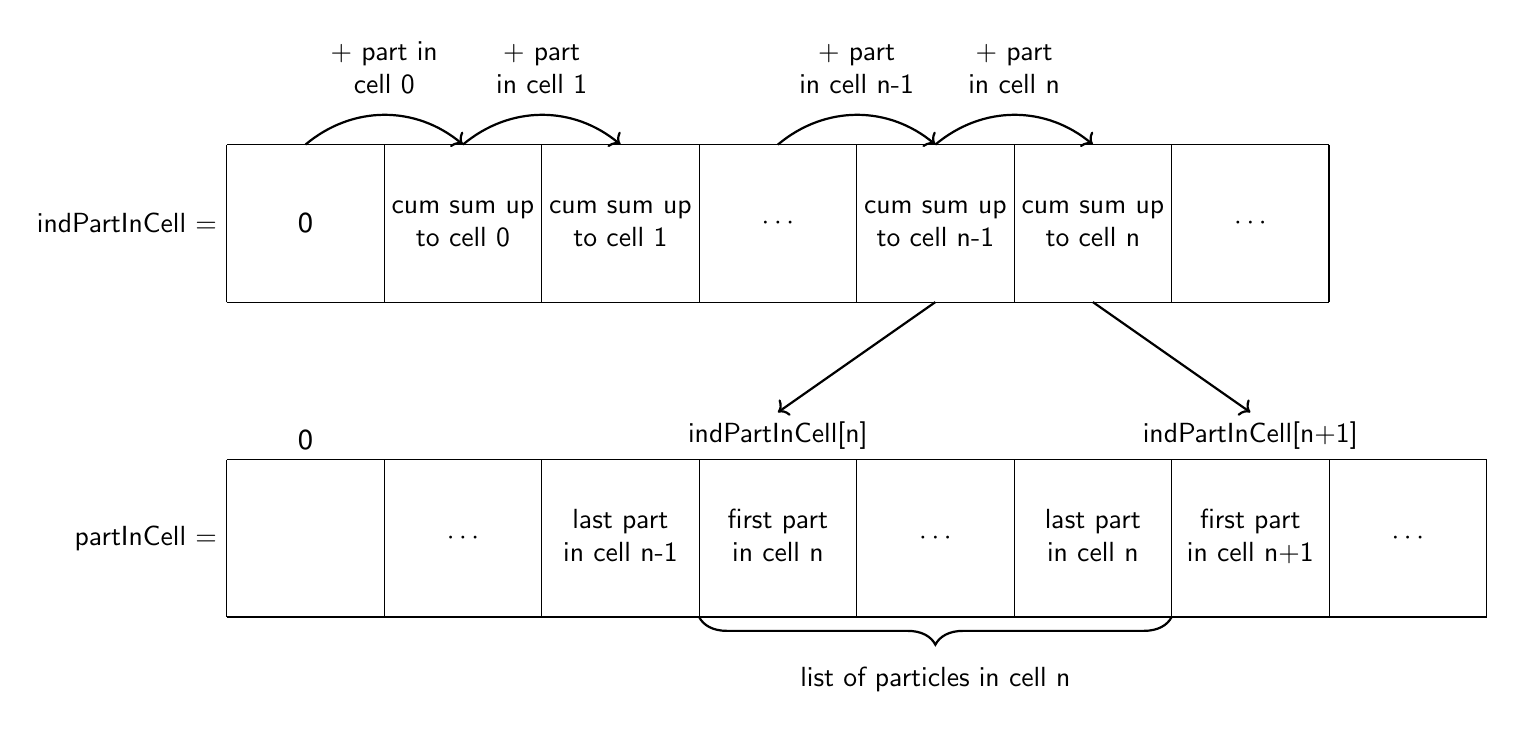
\begin{tikzpicture}[scale=2]
\def\y{0.5}
\draw (0,\y-0.5) grid (7,\y+0.5);

\draw (0,\y) node[left] {indPartInCell =};

\draw (0.5,\y) node {$0$};
\draw [thick,->] (0.5,\y+0.5) to [out=40,in=140] (1.5,\y+0.5);
\draw (1,\y+0.7) node[above] {\begin{tabular}{c} + part in \\ cell 0 \end{tabular}};
\draw (1.5,\y) node {\begin{tabular}{c} cum sum up \\ to cell 0 \end{tabular}};
\draw (2.5,\y) node {\begin{tabular}{c} cum sum up \\ to cell 1 \end{tabular}};
\draw [thick,->] (1.5,\y+0.5) to [out=40,in=140] (2.5,\y+0.5);
\draw (2,\y+0.7) node[above] {\begin{tabular}{c} + part \\ in cell 1 \end{tabular}};


\draw (3.5,\y) node {$\cdots$};
\draw [thick,->] (3.5,\y+0.5) to [out=40,in=140] (4.5,\y+0.5);
\draw (4,\y+0.7) node[above] {\begin{tabular}{c} + part \\ in cell n-1 \end{tabular}};
\draw (4.5,\y) node {\begin{tabular}{c} cum sum up \\ to cell n-1 \end{tabular}};
\draw [thick,->] (4.5,\y+0.5) to [out=40,in=140] (5.5,\y+0.5);
\draw (5,\y+0.7) node[above] {\begin{tabular}{c} + part \\ in cell n \end{tabular}};
\draw (5.5,\y) node {\begin{tabular}{c} cum sum up \\ to cell n \end{tabular}};
\draw (6.5,\y) node {$\cdots$};

\def\y{-1.5}
\draw (0,\y-0.5) grid (8,\y+0.5);

\draw (0,\y) node[left] {partInCell =};

\draw (0.5,\y+0.5) node[above] {$0$};
\draw (1.5,\y) node {$\cdots$};
\draw (2.5,\y) node {\begin{tabular}{c} last part \\ in cell n-1 \end{tabular}};
\draw (3.5,\y) node {\begin{tabular}{c}first part \\ in cell n \end{tabular}};
\draw (3.5,\y+0.5) node[above] {indPartInCell[n]};
\draw [thick,->] (4.5,0) -- (3.5,\y+0.8);
\draw (4.5,\y) node {$\cdots$};
\draw (5.5,\y) node {\begin{tabular}{c} last part \\ in cell n \end{tabular}};
\draw (6.5,\y+0.5) node[above] {indPartInCell[n+1]};
\draw [thick,->] (5.5,0) -- (6.5,\y+0.8);
\draw (6.5,\y) node {\begin{tabular}{c}first part \\ in cell n+1 \end{tabular}};
\draw (7.5,\y) node {$\cdots$};
\draw [thick,decorate,decoration={brace,amplitude=10pt,mirror}](3,\y-0.5) -- (6,\y-0.5) node[black,midway,yshift=-0.8cm] {list of particles in cell n};
\end{tikzpicture}
\end{document}
